\subsection{Connection setup in a busy network}
While the analysis performed in the connection setup test was performed on a network with no other activity, it is important to understand how network load affects performance.
In order to approximate load, a number of devices were configured to attempt a connection to a different device at a specified time.
Given that synchronization of wall-clocks is very hard to achieve on Android, the approach used was to instruct all the devices to initiate the connection after a fixed amount of time.
The script controlling the test computed the timeout so that all the devices started the connection at approximately the same time. 
Algorithm \ref{pseudo:script-collision} shows the pseudocode for the script controlling the simulation.

\begin{algorithm}
	\begin{algorithmic}[1]
  		\caption{script}
  		\label{pseudo:script-collision}
  		\State $devices \leftarrow [device_1 \dots device_n]$
  		\State shuffle($devices$)
  		\State $target \leftarrow devices[0]$
  		\State $others \leftarrow devices[1\colon]$ \Comment all the devices but the first
  		\State $delay \leftarrow 5 * 10^{8}$ \Comment 500 milliseconds
		\For{$device$ in $others$}
		    \State $T_0 \leftarrow nanotime()$ \Comment current time in nanoseconds
		    \State $device$.connectAfter($target$, $delay$)
			\State $T_1 \leftarrow nanotime()$
			\State $delay = delay - (T_1 - T_0)$
		\EndFor
		\State \Return collectResults($others$)
  	\end{algorithmic}
\end{algorithm}

\begin{figure}[ht!]
  \centering
  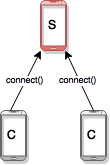
\includegraphics[width=0.2\textwidth]{application/img/collision.png} 
  \caption{To test the time required to open a connection in a loaded network, two client devices connected to a server device at the same time}
  \label{figure:collision}
\end{figure}

\begin{figure}[ht!]
  \centering
  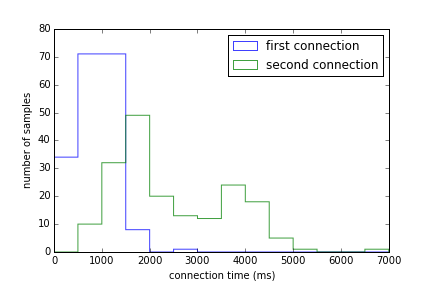
\includegraphics[width=1.0\textwidth]{application/img/collision_2.png}
  \caption{Distribution of connection times with 2 devices connecting to the target.}
  \label{figure:collision_2}
\end{figure}

\begin{figure}[ht!]
  \centering
  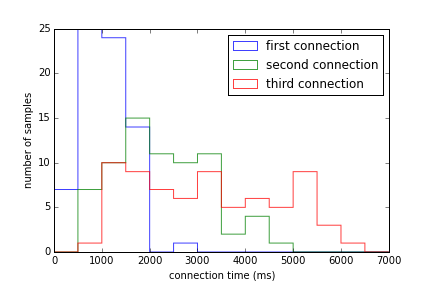
\includegraphics[width=1.0\textwidth]{application/img/collision_3.png}
  \caption{Distribution of connection times with 3 devices connecting to the target.}
  \label{figure:collision_3}
\end{figure}


\subsubsection{Test execution}
In order to collect a sufficient amount of data, the test was executed for a large number of times.
Table \ref{table:collision-failure-rate} shows the devices used along with the number of runs.

A single test randomly selected one of the devices as the target and used the others to perform the connections.
The connection time was then collected for each device $(CT_0 \dots CT_n)$ before the beginning of the following test. 
A test was considered successful when all the devices performed the connection without errors.


\begin{table}[h]
\centering
\caption{Failure rate for set of devices used}
\label{table:collision-failure-rate}
\begin{tabular}{lll}
\hline
Devices                             & Total     & Failed    \\ \hline
Nexus 4, Nexus 5, Nexus 7           & 350       & 162       \\
Nexus 4, Nexus 4, Nexus 5, Nexus 7  & 300       & 226       \\
\hline
\end{tabular}
\end{table}

\subsubsection{Results}
Figure \ref{figure:collision_2} and \ref{figure:collision_3} show the distribution of connection time obtained from the test with two and three devices respectively (excluding the target).

As shown in the figures, the increase in network load has a big impact on the connection time.
Moreover, the rate of failures showed in Table \ref{table:collision-failure-rate} suggest that multiple concurrent requests to the same device cause stability issues on the receiver.
